\chapter{Benchmarking and Result}

\section{Fine Tuning the Deep Learning Models}

On top of the five main dataset of size $> 20k$, DeepPrime has additional 18 datasets of size $\sim5k$, which were used to fine tune the model for better generalizability. As a result, for a more thorough comparison between the models, the same fine tuning process was conducted on all deep learning models.

To fine tune the models, the same hyperparameters were used as the original training, except for the learning rate, which was set to $1e-3$ for the fine tuning to accommodate the smaller dataset size. The sequence processing layers were frozen, leaving only the feature processing and the final meta learner to be trained. The models were trained for at most 300 epochs for each fold, and the best model was selected based on the validation loss.

\section{Benchmarking}

% TODO: add references to the section and appendix after including the results
As mentioned in section {ensemble training}, although both PRIDICT and DeepPrime uses different features, for a more direct comparison of the architecture, both models were retrained using the features selected from this study. Since all models use the same number of features (24), the data is hot swappable between the models, allowing for easier retraining if a more optimal feature set is found.

\section{Attention Analysis}
\label{sec:attention_analysis}

\begin{figure}
    \centering
    \subfigure[Substitution]{
        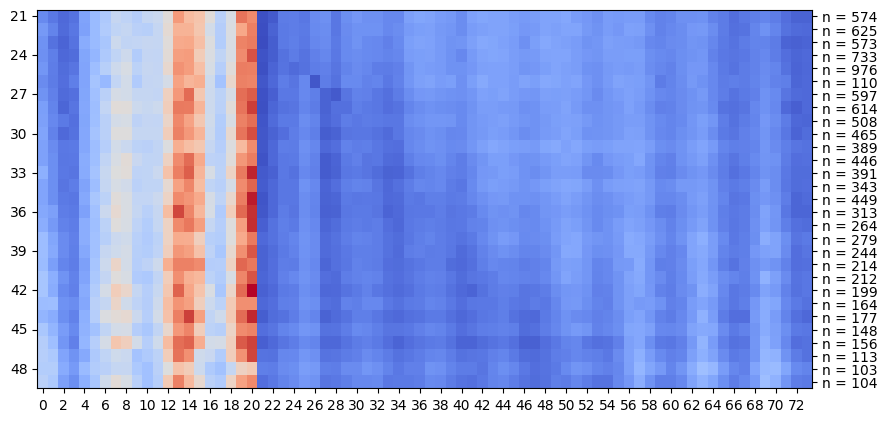
\includegraphics[width=0.9\textwidth]{dp-hek293t-pe2-transformer-only-attention-insertion.png}
        \label{fig:attention_insertion}
    }
    \subfigure[Insertion]{
        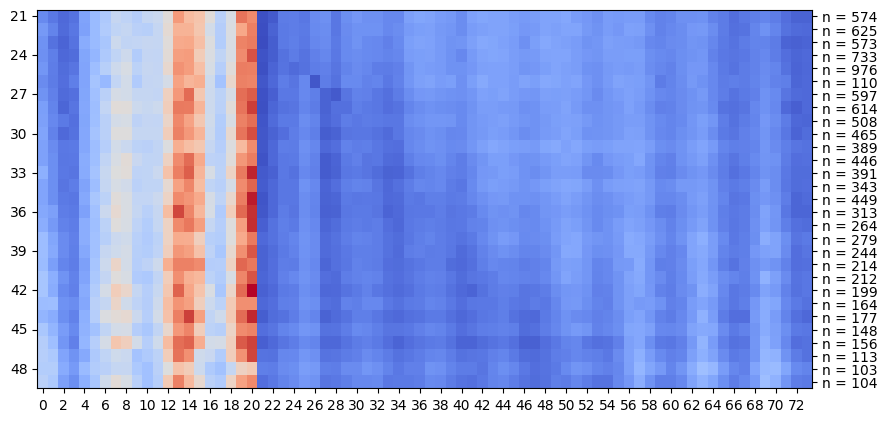
\includegraphics[width=0.9\textwidth]{dp-hek293t-pe2-transformer-only-attention-insertion.png}
        \label{fig:attention_substitution}
    }
    \subfigure[Deletion]{
        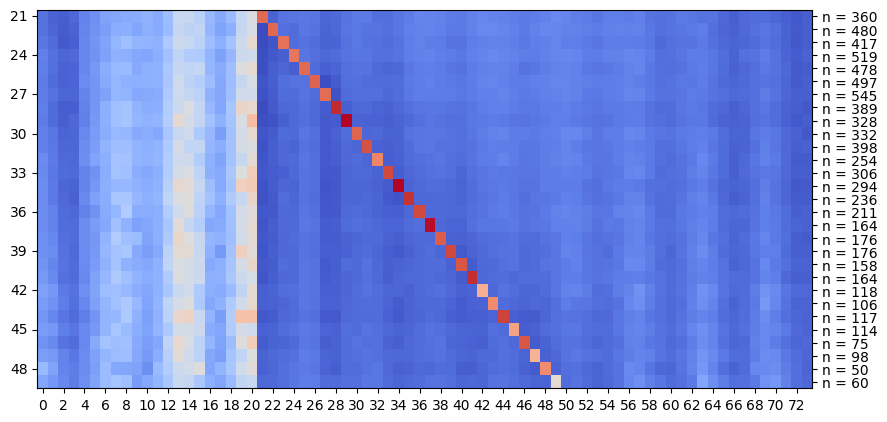
\includegraphics[width=0.9\textwidth]{dp-hek293t-pe2-transformer-only-attention-deletion.png}
        \label{fig:attention_deletion}
    }
    \caption[Attention weights for the DeepPrime model trained on the HEK293T-PE2 dataset]{Attention weights of length 1 edits for the DeepPrime model trained on the HEK293T-PE2 dataset. The x-axis represents the position of the transformer output token, the y-axis indicates the edit position. Red colour indicates higher attention weights, while blue indicates lower attention weights.}
    \label{fig:attention}
\end{figure}

A significant advantage of the attention based methods are their interpretability. The attention mechanism allows the model to focus on specific parts of the input data using the attention weights, which can be visualized teo understand the model's decision making process. 

In this architecture, the most informative and interpretable attention weights are the feature embedding attention weights at the final layer of the transformer model, pooling all token embeddings into a single feature embedding. 

The examples were grouped together by their editing type and length so that the edit positions can be easily identified and compared. And the attention weights for edits at the same position were aggregated to show the overall importance of the position in the editing efficiency prediction.

The model trained on the biggest DeepPrime dataset was first tested, as the transformer model has the greatest chance of learning the underlying motifs influencing the editing efficiency in the data. Starting with the edits of length 1, the attention weights were visualized for the substitution, insertion, and deletion, shown in \autoref{fig:attention}. 

However, for deletion, the attention weights were the highest at the edit position. The cross attention output of the edit position for deletion was dominated by the encoder output, as the self-attention weights for the mutated sequence at edit position were masked out to be zero. This is a possible indication that the model considers the base to edit as an important feature for the deletion operation.